\documentclass{midl} % Include author names
%\documentclass[anon]{midl} % Anonymized submission
\usepackage[british]{babel} % decent hyphenation, avoiding e.g. anal-ysis
\usepackage[iso]{isodate}
\usepackage{sansmath}
\usepackage{booktabs}
\usepackage{graphicx}
\usepackage{graphviz}
\usepackage{makecell}
\usepackage{minted}
\usepackage{multicol}
\usepackage{siunitx}
\usepackage{subcaption}
\usepackage[section]{placeins}

% Needs to be loaded after hyperref
\usepackage{cleveref}

% PythonTeX
\usepackage[autoprint=false, gobble=auto, keeptemps=all, pyfuture=all]{pythontex} % create figures on-line directly from python!
\usepackage{pgf}
%\input{/usr/share/repsep/functions.py}
\input{functions.py}
\begin{pythontexcustomcode}[begin]{py}
pytex.add_dependencies(
	'lib/utils.py',
	'lib/categorical.py',
	'data/JogB.tsv'
	)
\end{pythontexcustomcode}
% Single-session PythonTeX codeblocks
\newcounter{pysessioncounter}
\newcommand{\sessionpy}{%
          \edef\sessionpysession{session\arabic{pysessioncounter}}%
            \stepcounter{pysessioncounter}%
              \expandafter\py\expandafter[\sessionpysession]}

% SIunitx customizations detect-all will use the current font for typesetting
\sisetup{per-mode=symbol, detect-all, range-units = single}
\newcommand\SIci[5]{\SI{#1}{#2}, {#3}CI: \SIrange{#4}{#5}{#2}}

% Fix for matplotlib PGF wonkiness which isn't interpreted correctly by pdflatex
\DeclareUnicodeCharacter{2212}{-}

% The following packages will be automatically loaded:
% jmlr, amsmath, amssymb, natbib, graphicx, url, algorithm2e
% ifoddpage, relsize and probably more
% make sure they are installed with your latex distribution

\usepackage{mwe} % to get dummy images

% Header for extended abstracts
\jmlrproceedings{MIDL}{Medical Imaging with Deep Learning}
\jmlrpages{}
\jmlryear{2021}

% to be uncommented for submissions under review
\jmlrworkshop{Short Paper -- MIDL 2021 submission}
\jmlrvolume{-- Under Review}
\editors{Under Review for MIDL 2021}

\title[Multimodal Generative Learning on the MIMIC-CXR Database]{Multimodal Generative Learning on the MIMIC-CXR Database}


% More complicate cases, e.g. with dual affiliations and joint authorship
\midlauthor{\Name{Hendrik Klug\nametag{$^{1}$}} \Email{klugh@ethz.ch}\\
\addr $^{1}$ Institute for Electrical Engineering, ETH Zürich \\
\Name{Thomas M. Sutter\midlotherjointauthor\nametag{$^{2}$}} \Email{thomas.sutter@inf.ethz.ch}\\
\addr $^{2}$ Department of Computer Science, ETH Zürich \AND
\Name{Julia E. Vogt\nametag{$^{2}$}} \Email{julia.vogt@inf.ethz.ch}\\
}

\begin{document}

\maketitle
\begin{abstract}
    Machine Learning (ML) has become more and more popular in the medical domain over the past years.
    While supervised machine learning has received the most attention, unsupervised learning has great potential since there is more data available for the training of the models.
    Especially when leveraging the multi-modal nature of most clinical data, self-supervised learning can provide results comparable to supervised methods.
    Multi-modal unsupervised methods have been tested extensively on toy-datasets like MNIST \cite{lecun-mnisthandwrittendigit-2010, thomas_gener-ELBO, wu2018multimodal} and CelebA \cite{liu2015faceattributes, thomas_gener-ELBO, wu2018multimodal} but to the best of our knowledge have never been applied to medical data, for direct applications such as disease classification and image generation.
    In this article, we apply a method for self-supervised training proposed in \cite{thomas_gener-ELBO} to medical data from the MIMIC-CXR Database \cite{johnson2019mimic} and show that these methods provide promising results on medical data from the MIMIC-CXR database, while highlighting that the task is extremely challenging and that there is space for substantial improvements.
\end{abstract}


\begin{keywords}
Multimodal Learning, Generative Learning, VAE
\end{keywords}

\section{Introduction}

	Manually creating annotations of sufficient training examples for the training of a deep learning model is often infeasible, since it requires manual expert input.
	In the medical domain especially, human labeled data is expensive to acquire and thus very scarce.
	A generative model, that can learn embeddings of the data without the need for labels, enjoys a much bigger variety of possible training data.
	The Variational Autoencoder (VAE) \cite{doersch2016tutorial} in particular is a popular generative model, which consists of an encoder that maps the input to a learned latent distribution from which the decoder part samples to reconstruct the input.

	Clinical data comes in many modalities, such as images, text reports and electronic health records.
	A generative model that can leverage all of the modalities could be used for tasks such as generating a text report when given images of a patient, generating an image of another angle from an input image or data classification.
	However, in contrast to toy datasets, the different pathologies that represent the classes in medical data are defined by very subtle features that only human experts can recognise.
	This makes the task of learning a latent representation of the data, while preserving the separability of the classes extremely challenging.
	
	In this work, we apply the generalised multimodal ELBO, proposed in \cite{thomas_gener-ELBO}, to train a self-supervised, generative model on clinical data from the MIMIC-CXR Database \cite{johnson2019mimic} containing chest-X rays and related text reports. 
	We provide a first insight into the difficulties and opportunities that come with medical data.

\section{Methods}
Assuming the data consists of $N$ i.i.d. samples $\{\xseti\}^N_{i=1}$, each of which is a set of M modalities $\mathbb{X}^{(i)} = \{\textbf{x}_j^{(i)}\}^M_{j=1}$, the joint posterior distribution is calculated in two steps.
In a first step, a distribution is calculated for each subset of the powerset $\powerset$ using a Product of Experts (PoE) \cite{wu2018multimodal}.
In a second step these subsets are merged using a Mixture of Experts (MoE) \cite{shi2019variational} into a joint posterior distribution.

The MIMIC-CXR Database \cite{johnson2019mimic} provides a class-label for every sample, corresponding to one or more of 13 pathologies.
For the evaluation of our method, we created a label "Finding", indicating if the sample is labeled with any of the 13 pathologies. 
All images were resized to (128, 128) and every word that occurs at
least 3 times in all the text reports is mapped to an index. 
Using this mapping each sentence is encoded into a sequence of indices. 
All sentences with a word count above 128 are truncated and all sentences consisting of less words are padded with a padding token "$< pad>$" such that all text samples are of length 128.

\section{Results}

    In the following section, we will abbreviate the three modalities present in the data selection with "F" for frontal scan, "L" for lateral scan and "T" for text report.
    
    \subsection{Evaluation of the latent representation}
    
    
    %The random performance lies at \py{boilerplate.read_rand_perf()}.\\
    
    \Cref{tab:lr_table_bin} shows the evaluation of the linear classifiers that were trained on the learned latent representation.
    We note that the uni-modal subspaces provide a less good separability between samples that are labeled with a Finding and samples that are not.
    Especially when adding information of the T and the F subspaces does the classification score increase.
    While the information of the L subspace does not improve the classification score when added to the other image modality F, it does significantly increase the score when added to the text modality T.
    The highest score is achieved by the classifiers evaluated on the T and the F modality.
    Overall, the text modality provides the best separability.
    This is expected since the text modality is the easier modality to learn from because it contains the label assignment encoded in a much simpler manner than for the image modalities.
    The text reports of samples belonging to a certain label will contain that label in their text.
    
    \Cref{tab:clf_table_bin} shows the mean average precision score of the supervised method on the same test set.
    Overall the classifiers trained with manually labeled data achieve higher scores for all modalities.
    This difference in performance can be explained by the different training objectives of the two methods.
    The supervised classifiers were trained with the objective of classifying the samples correctly.
    This comes at the cost of needing a sufficiently big dataset with samples that need to be annotated by an expert in the case of medical data.
    The classification ability of the unsupervised method on the other hand, is simply a byproduct of the learning of a latent representation of the data.
    
    \py{
        pytex_tab(
        script='scripts/lr_table_bin.py',
        label='lr_table_bin',
        caption='\\textbf{Classification results of the linear classifiers trained on the learned latent representation using the binary label "Finding"}. The mean average precision over the test set is reported for each modality (F: frontal scan, L: lateral scan, T: text report). The classifiers evaluated on the subspace containing all modalities achieves the highest mean average precision.',
        options_pre='\\centering \\resizebox{0.9\\textwidth}{!}{',
        options_post='}',
        )
    }
    
    
    \py{
        pytex_tab(
        script='scripts/clf_table_bin.py',
        label='clf_table_bin',
        caption='\\textbf{Classification results of the supervised classifiers using the binary label "Finding"}. The mean average precision over the test set is reported for each modality (F: frontal scan, L: lateral scan, T: text report). The classifier trained on the T modality achieves the highest score.',
        options_pre='\\centering \\resizebox{0.5\\textwidth}{!}{',
        options_post='}',
        )
    }
    
    
    %\py{
    %    pytex_tab(
    %    script='scripts/lr_table.py',
    %    label='lr_table',
    %    caption='\\textbf{Classification results of the linear classifiers trained on the learned latent representation using the binary label "Finding"}. The mean average precision over the test set is reported for each modality (F: frontal scan, L: lateral scan, T: text report). The classifiers evaluated on the subspace containing all modalities achieves the highest mean average precision.',
    %    options_pre='\\centering \\resizebox{0.9\\textwidth}{!}{',
    %    options_post='}',
    %    )
    %}
    %
    %\py{
    %    pytex_tab(
    %    script='scripts/clf_table_new.py',
    %    label='clf_table',
    %    caption='\\textbf{Classification results of the supervised classifiers using the binary label "Finding"}. The mean average precision over the test set is reported for each modality (F: frontal scan, L: lateral scan, T: text report).',
    %    options_pre='\\centering \\resizebox{0.7\\textwidth}{!}{',
    %    options_post='}',
    %    )
    %}
    
    \subsection{Evaluation of the generation coherence}
    
    Here we evaluate if the model, given input samples, is able to generate coherently.
    The generation is said to be coherent if the generated classes are classified to the same class as the input samples.\\
    \Cref{tab:gen_eval_table} shows the results values of the generation coherence of the MoPoE.
    Overall, the generated samples of the F modality provide the best generation coherence and adding other modalities as conditioner does not have a significant impact on the score.
    
    \Cref{fig:fig_cond_lattext} and \cref{fig:fig_cond_latPAtext} compare the generation quality of the model, without the F modality as input as well as given the F modality as conditioner.
    Adding the F modality as input for the generation brings a significant improvement to the quality of the generated samples.
    The generated samples from \cref{fig:fig_cond_latPAtext} are less blurry and smaller details are recognizable.
    We note that while the text modality is the modality that provides the best performance in the evaluation of the latent representation, it hard for the model to generate text samples given only the image modalities.
    It is however capable to copy the input text, when the text modality is given as conditioner.
    
    
    \begin{figure}
        \centering
        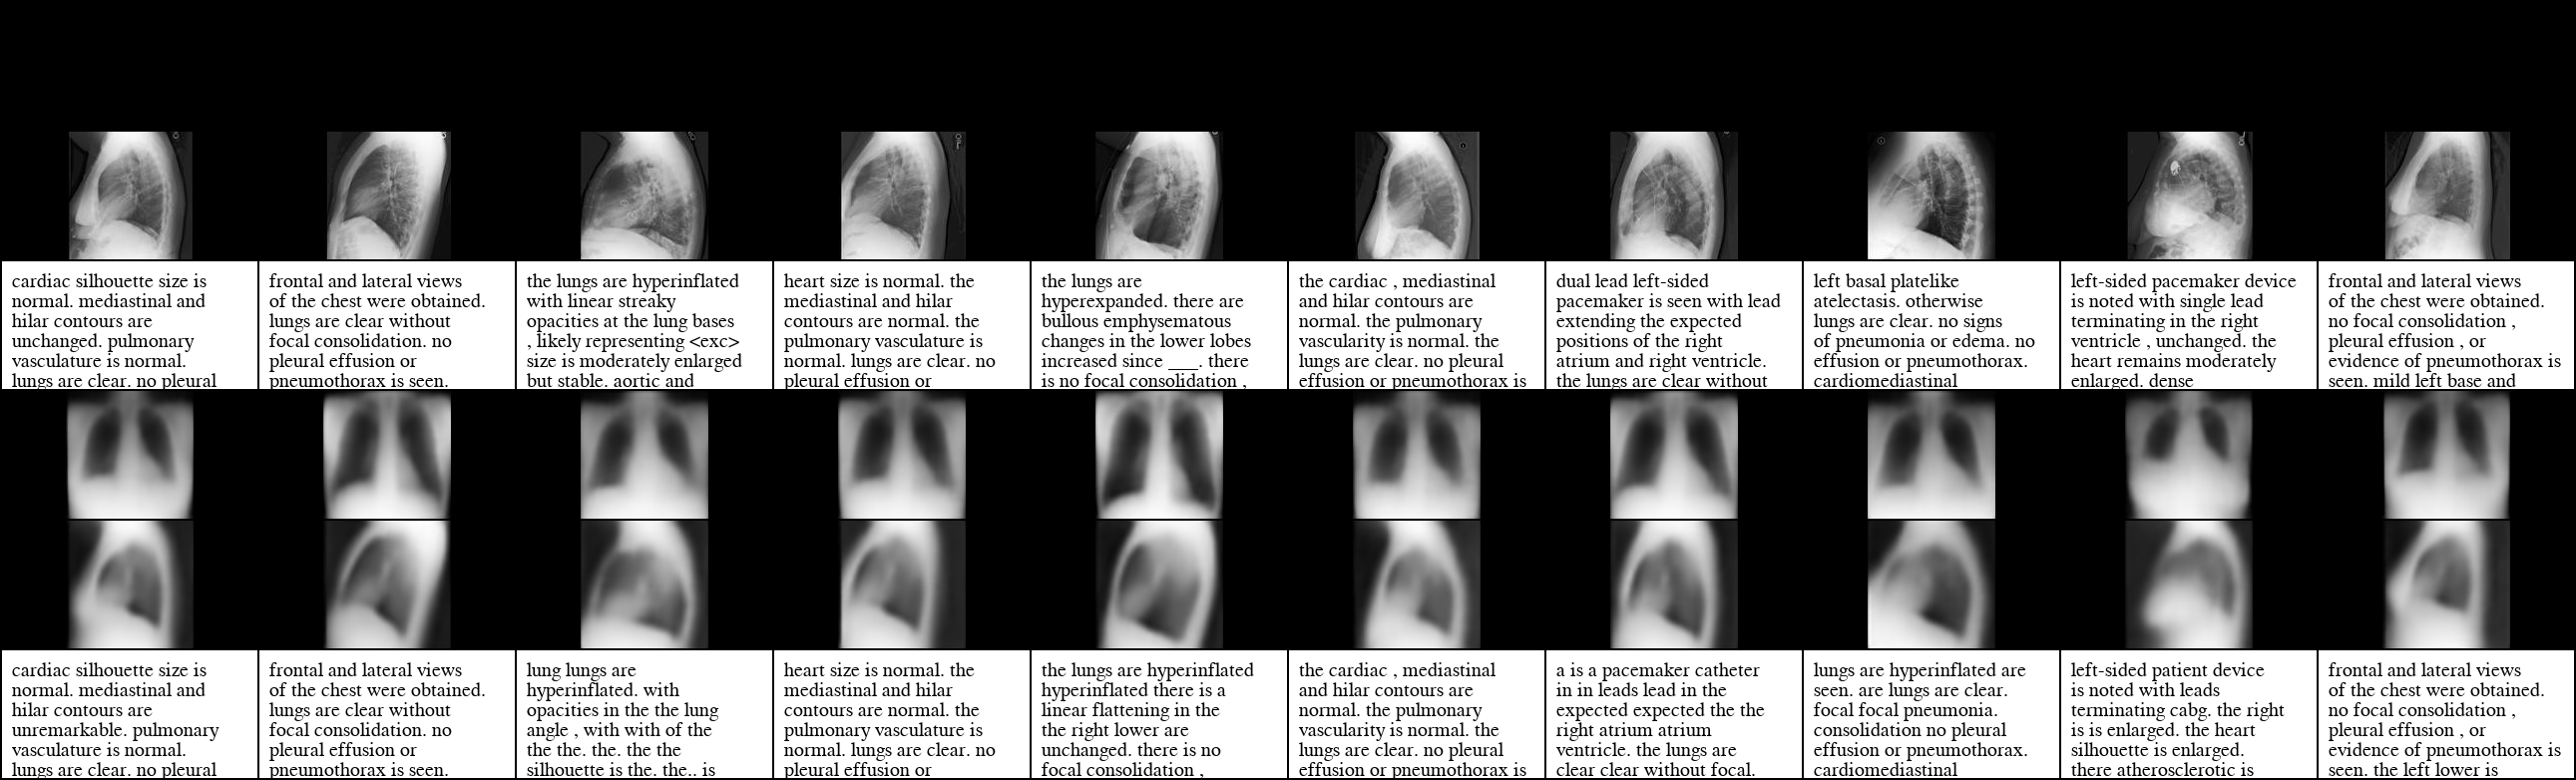
\includegraphics[width=\textwidth]{data/cond_gen/Lateral_text}
        \caption{
            \textbf{Conditionally generated samples with F and T modalities as conditioner.} The second and third image rows were given to the model as conditioner. The three last images rows are the generated samples. The images in the first row are the scans that correspond to the samples given as conditioner. The generated samples are blurry and it is difficult to see whether they represent some of the features that are characteristic to the input samples.
        }
        \label{fig:fig_cond_lattext}
    \end{figure}
    
    \begin{figure}
        \centering
        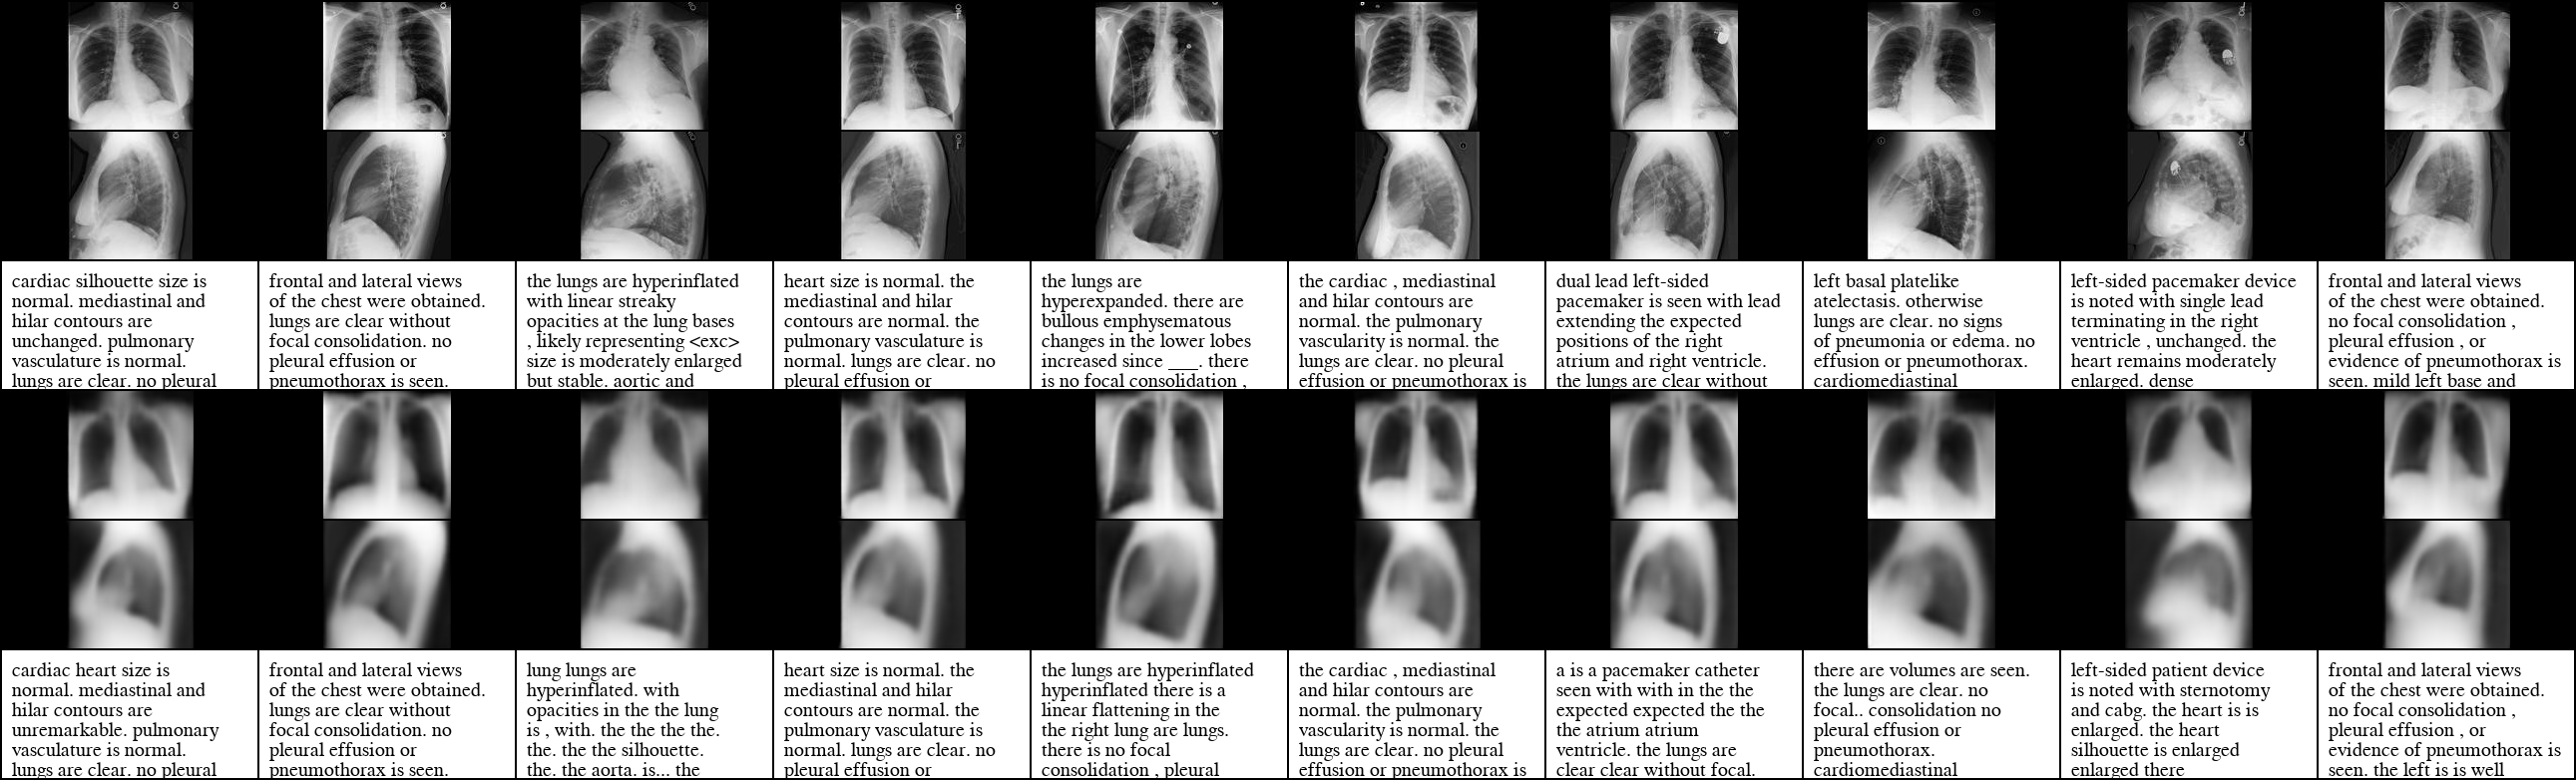
\includegraphics[width=\textwidth]{data/cond_gen/Lateral_PA_text}
        \caption{
            \textbf{Conditionally generated samples with F, L and T modalities as conditioner.} While the generated images are blurry, they do present some features that can be found in the input samples.
        }
        \label{fig:fig_cond_latPAtext}
    \end{figure}
    
    
    \py{
        pytex_tab(
        script='scripts/gen_eval_table.py',
        label='gen_eval_table',
        caption='\\textbf{Evaluation of the generation coherence.} For conditional generation, the letter below the horizontal line indicates the modality which is generated based on the input subsets $\\xset _k$ above. We report the mean average precision values between the prediction of a trained classifier on the generated samples and the label of the input samples.',
        options_pre='\\centering \\resizebox{0.9\\textwidth}{!}{',
        options_post='}',
        )
    }

\section{Conclusion}
    In this work, we applied a multi-modal generative model on clinical data to evaluate its performance on direct applications in the medical field.
    
    While our experiments show promising results, they indicate that the task is extremely challenging with significant scope for improvement.
    
    In particular, we showed that features in medical scans that are characteristic of most diseases are often smaller details that get lost in the blurriness of the generated samples.
    However, the latent representation that the MoPoE learns when learning to reproduce the data is still meaningful in the sense that it can be separated into the different classes the data belong to.

    While the learning of this representation was done in a supervised manner, the evaluation of the separability used handcrafted labels.
    Having shown that the latent space learned by the MoPoE is separable, it would be interesting to see if it can be separated in an unsupervised manner such as a clustering method.
    This would make the MoPoE a fully unsupervised classifier that we believe would perform better than a clustering method on raw, high dimensional medical data.
    The more complex loss function from our method can incorporate more prior knowledge and impose regularization.
    
    
    We have shown that the text modality provides the best separability of the latent representation but is also the most difficult to generate.
    This indicates that further research into the text decoder architecture could increase the performance of the method.
    
    
    
    We argue that our method is a successful first step into creating an unsupervised method that will find applications in the medical domain such as classification of diseases, generating text reports from medical data and generating scans from multiple angles.
    However, we believe that the method can be improved with some further fine-tuning, for example in the choice of the abstract mean function for modelling the joint posterior or in the choice of the encoder-decoder architectures.


% Acknowledgments---Will not appear in anonymized version
\midlacknowledgments{We thank a bunch of people.}


\bibliography{bib}


\appendix

\section{Proof of Theorem 1}

This is a boring technical proof of
\begin{equation}\label{eq:example}
\cos^2\theta + \sin^2\theta \equiv 1.
\end{equation}

\section{Proof of Theorem 2}

This is a complete version of a proof sketched in the main text.

\end{document}